\section{準備}
\label{section: preliminaries}

\subsection{表記}
(二進)自然数の集合を $\N$, 整数の集合を $\Z$, 実数の集合を $\R$, 
有理数の集合を $\Q$, $\T = \{0^n \mid n \in \N\}$ と表記する. 

一変数関数 $f:[0,1] \to \R$ が $i$ 回微分可能であるとき,
その $i$ 階導関数を $\D{i}f$ と表記する.
同様に二変数関数 $g$ の第一変数にたいして $i$ 階, 第二変数にたいして $j$ 階の導関数を $\D{i,j}g$ と表記する.

\subsection{実数の名}
 実数は無限の長さを持つため, 有限な文字列に符号化することが不可能である.
 そこで実数を計算可能なモデルで扱うために, 
 求める精度を与えると, 実数の近似値をその精度で返すような関数を考える.

\begin{definition}[実数の名]
 関数 $\phi : \T \to \Z $ が実数 $x \in [0,1]$ の名であるとは,
 $\phi(0^n) = \lfloor x \cdot 2^n \rfloor$ または
 $\phi(0^n) = \lceil x \cdot 2^n \rceil$ を満たすこと.
\end{definition}

\subsection{計算可能実関数, 多項式時間実関数}
 実関数は入力として実数を受け取るが, 実数を符号化することは不可能である.
 そこで入力の実数は神託として与える.
 そして実関数のモデルを, 求める精度を入力として受け取り
 関数の入力である実数の名を神託とし, 関数の値の近似値を返すような神託機械として定義する
 [図 \ref{fig:model-of-function}].
 より厳密には以下のように定義する.

 \begin{figure}
  \label{fig:model-of-function}
  \begin{center}
   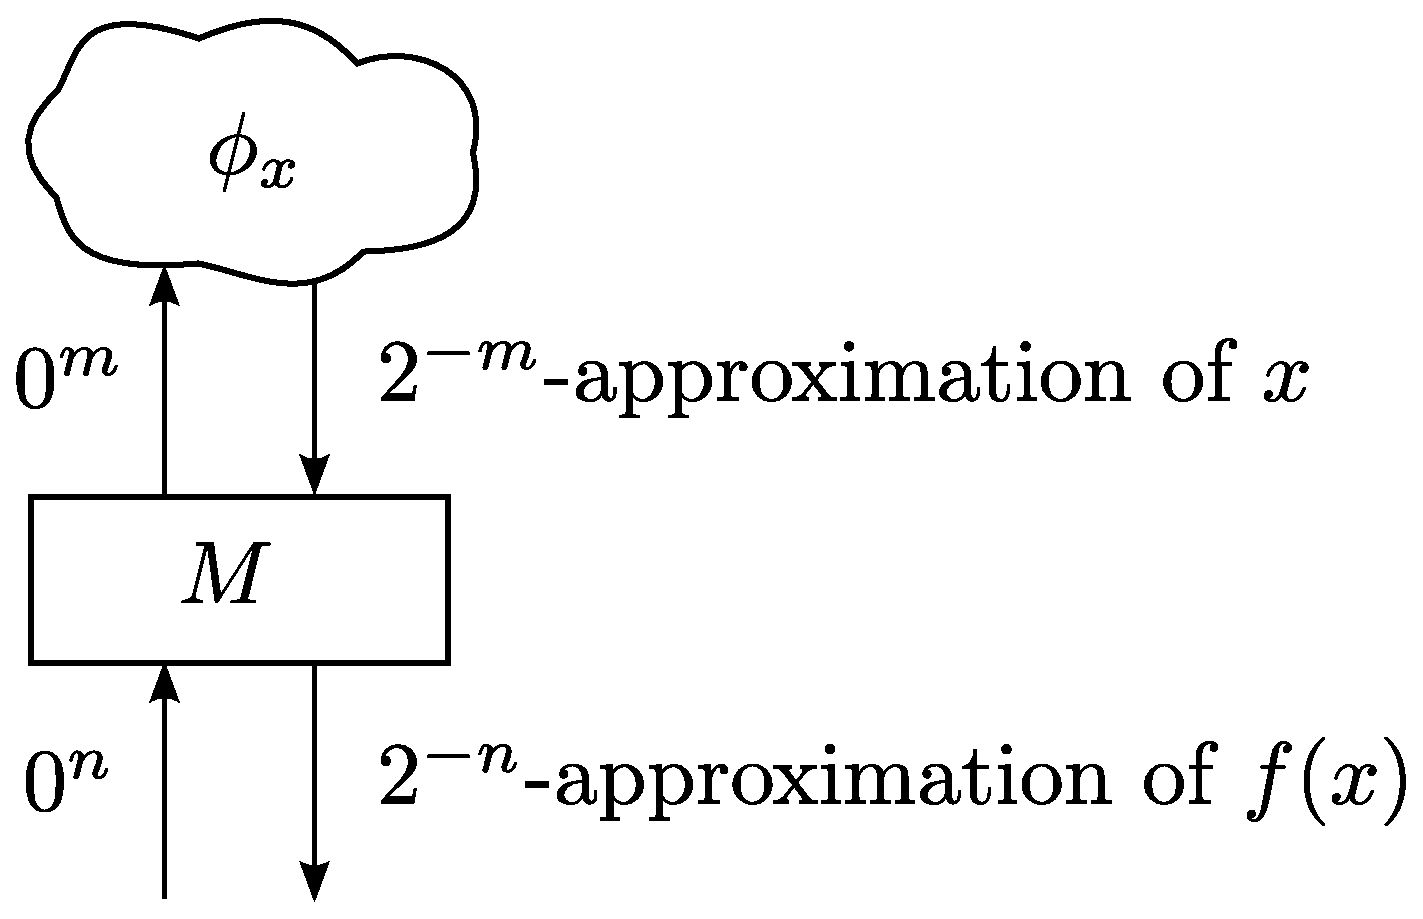
\includegraphics[height=0.15\textheight]{image/model-of-function.eps}
  \end{center}
  \caption{実関数のモデル化}
 \end{figure}

 \begin{definition}
  神託機械 $M$ が実関数 $f:A \to \R$ を計算するとは,
  任意の実数 $x \in A$, 任意の $x$ の名 $\phi_x$ にたいして,
  $M^{\phi_x}$ が $f(x)$ の名であること.
 \end{definition}

 多変数関数のモデルも, 変数と同じ数だけ神託を持つ神託機械によって同様に定義される.

 ある実関数が計算可能であるとは, その関数を計算する神託機械が存在することである.
 同様に, ある実関数が多項式時間計算可能であるとは, その関数を計算する多項式時間神託機械が存在することである.

 神託機械 $M$ がある実関数族 $(f_u)_u$ を計算するとは,
 入力 $u$ を受けったとき, $M_u$ が $f_u$ を計算することである.
 実関数族が多項式時間計算可能であるとは, その実関数族を計算する
 多項式時間神託機械が存在することである.
 

 神託機械 $M$ で $f$ を計算するとき, 求める精度 $n$ にたいして,
 $x$ の近似値に必要な精度 $m$ が定まるため,
 計算可能な関数は連続である.
 また $n$ と $m$ の対応関係と有理数における近似値を与えることで,
 計算可能実関数や多項式時間計算可能実関数にたいして,
 神託機械を用いない同値な特徴付けが可能である.

 \begin{lemma}
  実関数 $f:[0,1] \to \R$ にたいして,
  $\phi_f: (\Q \cap [0, 1]) \times \T \to \Q$, $m_f: \N \to \N$は
  \begin{align}
   |\phi_f(d, 0^n) - f(d)| \le 2^{-n} 
   &\qquad (d \in (\Q \cap [0,1]), \quad n \in \N)\\
   |x-y| \le 2^{-p_f(m)} \Rightarrow |f(x) - f(y)| \le 2^{-m}
   &\qquad (x, y \in [0, 1], \quad m \in \N)
  \end{align}
 をみたす関数とする.
  \begin{itemize}
   \item $f$ が計算可能であることは, 計算可能な $\phi_f, m_f$ が存在することと同値である. 
   \item $f$ が多項式時間計算可能であることは, 多項式時間計算可能な 
  $\phi_f$, 多項式 $m_f$ が存在することと同値である.
  \end{itemize}
\end{lemma}

\subsection{完全性}

 関数の下限を示すために, 困難及び完全性を定義する.
 言語 $L$ が実関数 $f:[0,1] \to \R$ に多項式時間還元可能であるとは,
 $f$ を計算する機械をブラックボックスとして, 入力 $u$ にたいして,
 精度を $f$ に与え, ある実数 $x_u$ の神託を模倣し, $f(x_u)$ の近似値から,
 $u$ が $L$ に含まれるか否かを多項式時間で計算可能であることである
 [図 \ref{fig:reduction}].
 厳密には以下のように定義する.

 \begin{definition}[多項式時間還元可能]
  言語 $L$ が実関数 $f:[0,1] \to \R$ に多項式時間還元可能であるとは, 
  任意の文字列 $u$ にたいして, 以下を満たす実数 $x_u \in [0,1]$
  多項式時間計算可能な関数 $R,S,T$ が存在すること.
  \begin{itemize}
   \item $R:N \times N \to \{0,1\}, \quad S:\N\times \T \to \N, \quad
  T:\N \to \T$;
   \item $S(u, \cdot)$ は実数 $x_u$ の名;
   \item 任意の $f(x_u)$ の名 $\phi$ にたいして
	 \[
	  L(u) = R(u, \phi(T(u))).
	 \]
  \end{itemize}
 \end{definition}

 \begin{figure}
  \begin{center}
  \label{fig:reduction}
  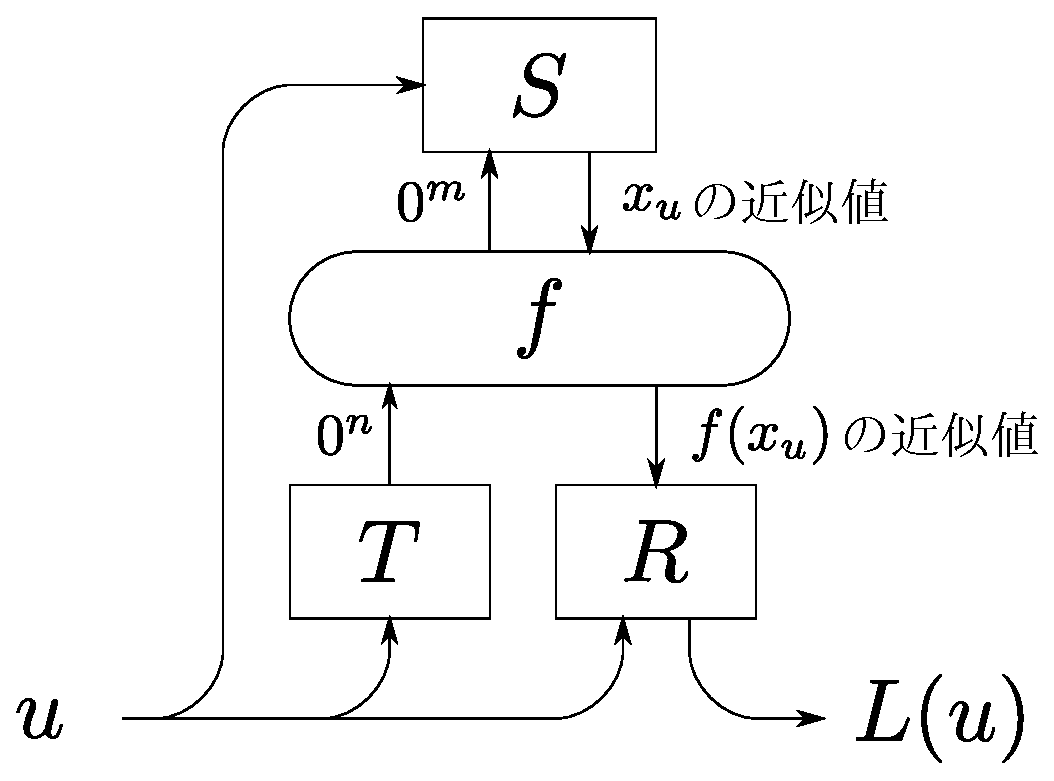
\includegraphics[height=0.2\textheight]{image/reduction.eps}
  \caption{言語 $L$ から関数 $f$ への還元}
  \end{center}
 \end{figure}

 計算量 $C$ にたいして, 関数 $f$ が $C$困難であるとは,
 任意の $C$ に含まれる言語が $f$ に多項式時間還元可能であることである.
 さらに $f$ が $C$ に含まれるとき, つまり $C$ に対応する神託機械で $f$ を計算するものが
 存在するとき, $f$ は $C$ 完全であると定義する.
 
